\section{Testes}
Vários testes foram implementados para que a geração de código de desvio para expressões booleanas, realizada pelo compilador, fosse avaliada. Os testes a seguir mostram a sensitividade do \textit{front end} em relação ao seguintes erros:
\begin{enumerate}
\item Erros de sintaxe.
\item Erros de tipo.
\item Erros de declarações inexistentes.
\item Erros de uso inadequado de tipos em condições (if, do, while).
\end{enumerate}

Antes de elucidar a capacidade de retornar erros quando necessário, mostraremos o funcionamento padrão e correto para um programa fonte de acordo com a linguagem \textbf{SmallL}:

\begin{lstlisting}[language=C, caption=Teste com entrada sem erros.]
{
    int i; int j; float v; float x; float[100] a;
    while( true ) {
        do i = i+1; while( a[i] < v);
        do j = j-1; while( a[j] > v);
        if( i >= j ) break;
        x = a[i]; a[i] = a[j]; a[j] = x;
    }
}
\end{lstlisting}

A saída é retornada sem erros, gerando as quadruplas identificadas pelo \textit{front end}:

\begin{figure}[H]
    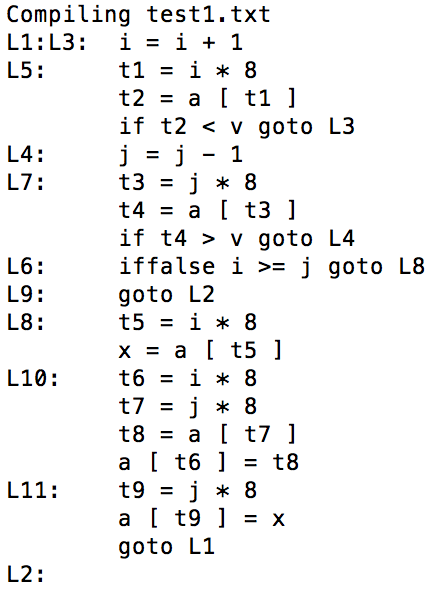
\includegraphics[width=.4\textwidth]{imgs/test1.png}
    \caption{Saída para entrada sem erros.}.
    \label{fig:dccnet}
\end{figure}

Nesta saída é possível identificarmos dois dos principais processos de geração no código intermediário: geração de código para expressões e para comandos. Na linha 1 temos o código gerado para expressão $i = i + 1$, composta por uma expressão aritmética de adição seguida de um comando de atribuição. Na linha 9 temos o código gerado para o comando \texttt{if( i >= j ) break}. A geração de código para declarações não é explícita pois elas resultam em entradas na tabela de símbolos para identificadores.

Nas seções a seguir mostraremos os testes para identificações de erros.

\subsection{Erro de sintaxe}

\begin{lstlisting}[language=C, caption=Teste de erro de sintaxe.]
{
    int a; char b;
    while {
        int c;
    }
}
\end{lstlisting}

O teste acima apresenta um erro de sintaxe após o comando \textbf{while} (não é apresentado sua condição). Tal situação configura um erro, segundo a gramática da linguagem. Logo, o \textit{front end} retorna erro, como pode ser observado abaixo:

\begin{figure}[H]
    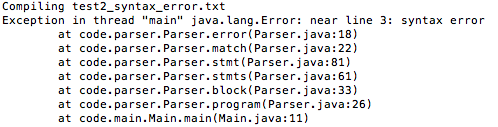
\includegraphics[width=1\textwidth]{imgs/test2.png}
    \caption{Saída para entrada com erros de sintaxe.}.
    \label{fig:test2}
\end{figure}


\subsection{Erro de tipo}

\begin{lstlisting}[language=C, caption=Teste de erro de tipo.]
{
  int a; char b; float c;
  a = 1;
  b = 2;
  if (a == b) {
    c = 0;
  }
}
\end{lstlisting}

Nesse teste são declaradas duas variáveis de tipos diferentes (int a e char b) e a seguir ambas são utilizadas na comparação do \textbf{if}. Tal situação não é válida segundo a linguagem \textbf{SmallL}. Portanto, o \textit{front end} retorna o erro abaixo:

\begin{figure}[H]
    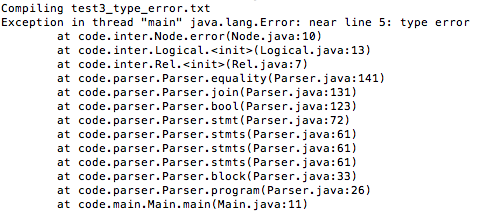
\includegraphics[width=1\textwidth]{imgs/test3.png}
    \caption{Saída para entrada com erros de tipo.}.
    \label{fig:test3}
\end{figure}


\subsection{Erro de declarações inexistentes}

\begin{lstlisting}[language=C, caption=Teste de declarações inexistentes.]
{
  float a;
  a = 4;
  if (b == 2){
    a = 5;
  }
}
\end{lstlisting}

Nesse teste usa-se uma variável (b) em uma condição do \textbf{if} que não foi declarada previamente. Tal situação representa um erro e o \textit{front end} identifica isso de forma correta, como mostra a saída abaixo:

\begin{figure}[H]
    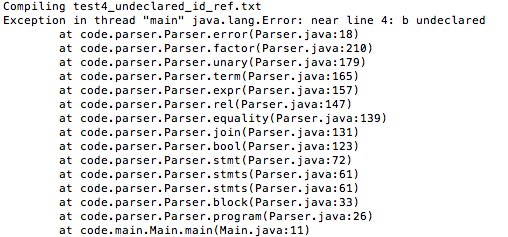
\includegraphics[width=1\textwidth]{imgs/test4.png}
    \caption{Saída para entrada com erro de declarações inexistentes.}.
    \label{fig:test4}
\end{figure}


\subsection{Erro de uso inadequado de tipos em condições}

\begin{lstlisting}[language=C, caption=Teste de uso inadequado de tipos em condições.]
{
    int a;
    int c;
    if (a){
        c = 2;
    }
}
\end{lstlisting}

Nesse teste é usado uma variável do tipo \textbf{int} (a) na condição do \textbf{if}, o que não é esperado de acordo com a gramática da linguagem. Logo, o \textit{front end} retorna um erro, como mostra a saída abaixo:

\begin{figure}[H]
    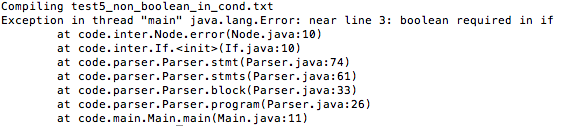
\includegraphics[width=1\textwidth]{imgs/test5.png}
    \caption{Saída para entrada com erro de uso inadequado de tipos.}.
    \label{fig:test5}
\end{figure}

